\documentclass[conference]{IEEEtran}
\IEEEoverridecommandlockouts
% The preceding line is only needed to identify funding in the first footnote. If that is unneeded, please comment it out.
\usepackage{cite}
\usepackage{amsmath,amssymb,amsfonts}
\usepackage{algorithmic}
\usepackage{graphicx}
\usepackage{textcomp}
\usepackage{xcolor}
\usepackage{url}
\usepackage{hyperref}
\usepackage{subcaption}
\def\BibTeX{{\rm B\kern-.05em{\sc i\kern-.025em b}\kern-.08em
    T\kern-.1667em\lower.7ex\hbox{E}\kern-.125emX}}
\graphicspath{{images/}}

\begin{document}

\title{Vehicle License Plate Recognition in Armenia\\
\textit{Spring 2023}}

\author{\IEEEauthorblockN{Author: Diana Sargsyan}
\IEEEauthorblockA{\textit{BS in Data Science} \\
\textit{American University of Armenia}\\
}
\and
\IEEEauthorblockN{Supervisor: Elen Vardanyan}
\IEEEauthorblockA{\textit{American University of Armenia} \\
}
}
\maketitle

\begin{abstract}
This capstone project presents an Automatic Number Plate Recognition (ANPR) system designed to detect and recognize Armenian license plates. The system employs an object detection algorithm to detect license plates, applies skew and rotation adjustment to correct the orientation, and uses optical character recognition to recognize the characters on the plate. The project achieves a high accuracy rate of 90\verb|%| on plate detection and 95\verb|%| on character recognition on a manually collected dataset consisting of high-quality photos and videos. Overall, this project presents a promising solution for ANPR systems.
\end{abstract}

\section{Introduction}

Automatic License/Number Plate Recognition (ANPR/ALPR) is a computer vision-based system that has gained high popularity over the last few years due to its ability to recognize license plates of vehicles and provide multiple valuable applications such as traffic law enforcement, parking enforcement, retail park security, and tolling.
Automatic Number Plate Recognition takes an image or video as an input and detects vehicle license plate numbers. 
An ANPR system is typically comprised of the following steps:
\begin{enumerate}
    \item Detection and localization of a license plate from a vehicle image or frame.
    \item Skew and rotation adjustment.
    \item Character recognition.
\end{enumerate}

The motivation behind this capstone project was to develop an ANPR system for Armenian license plates. Upon thorough research on automatic plate detection, there were no datasets available for Armenian license plates. 

After thorough research of the available number plate recognition techniques, this project presents a system that uses an object detection algorithm to identify license plates from a given image or a video, applies preprocessing techniques to fix the orientation of the license plate, and applies an optical character recognition program to output the license plate characters from the image. 
The \textbf{Tools} section of this paper presents the specific software and hardware resources utilized to complete the project. The \textbf{Data} section provides information about the data collection methodology and any preprocessing conducted. The \textbf{Literature Review} section presents an overview of existing research and relevant literature. The \textbf{Plate Detection} section details the techniques employed to detect and localize license plates in images or video frames. The \textbf{Skew Adjustment} section thoroughly explains the detection and correction of rotation in license plate images. The \textbf{Character Recognition} section focuses on recognizing the characters on the license plate after the localization and skew adjustment processes. The \textbf{Video Detection and Recognition} section provides detailed information on how the system was applied to videos. The \textbf{Results and Discussion} section assesses the accuracy of the ANPR system and concludes the findings. Finally, the \textbf{Conclusion and Future Work} section outlines potential improvements for the proposed solution.

\section{Tools}

\textbf{LabelImg}, an annotation tool was used to prepare the data. The research project utilized \textbf{YOLOv7} to perform object detection with high accuracy. The detection algorithm can identify license plates on images and videos, providing the competence needed for an ANPR system. Python was chosen as the programming language for its user-friendly features. \textbf{Google Colaboratory} was used for its free access to GPUs. It also has no setup requirements, making it effortless to use and significantly speeding up the training process for plate detection. \textbf{Jupyter Notebook} was used to document the project interactively. \textbf{OpenCV} (Open Source Computer Vision), an image processing library, was used for its extensive library of image and video processing functions. \textbf{EasyOCR} was also utilized for its optical character recognition purpose to recognize the numbers and letters on the extracted and preprocessed license plates. 

\section{Data}
\subsection{Image Data}

Given that there are few datasets related to Armenia, one of the motivations for this project was to accumulate an Armenian license plate dataset. Collecting a custom dataset in Armenia will allow future researchers to reproduce and use the existing data in their projects and, most importantly, contribute to the large gap in data availability in Armenia. The dataset used in this project was manually collected by taking pictures of vehicles in different locations in Yerevan and consists of 170 images. A video is also available in the project repository for experimentation of the system on a video.  

\subsection{Label Data}

To detect license plates from an image, there needs to be a corresponding .txt file that contains the coordinates of the number plate. An open-source graphical image annotation tool called "LabelImg" was used to gather these coordinates. The tool provides data in Pascal VOC, YOLO, and Tensorflow formats after users draw bounding boxes to mark the object they want to detect from an image \cite{b1}. In this case, the bounding box is placed over the license plates.

\begin{figure}[h]
    \centering
    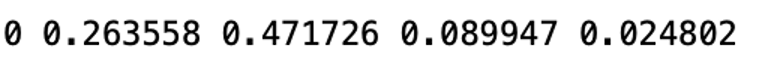
\includegraphics[width=0.4\textwidth]{images/Picture1.png}
    \caption{Example of a LabelImg-generated .txt label file for object detection.}
    \label{fig:Picture1}
\end{figure}

The labeled data is saved as .txt or . xml files with the same name as the image used to annotate over. LabelImg also saves a classes.txt file with the name of the class being identified. An example of a labeled .txt file can be seen in Figure \ref{fig:Picture1}. This project has only one class because only one object: a license plate, is being detected. The first integer in the label file represents the object class number, starting from 0 instead of 1. The following two numbers correspond to the x and y coordinates of the bounding box, while the fourth and fifth numbers represent the width and the height of the bounding box, respectively \cite{b1}.

\section{Literature Review}

Many solutions have been proposed and applied to the problem of ANPR in computer vision and image processing. 
Kaur et al. \cite{b2} proposed approaching license plate localization by implementing training on the object detection model YOLOv5. 
YOLO is a widely used object detection algorithm, first released in 2016 but has since had many developments made to it and released multiple new versions.
Currently, the 7th version release of YOLO is considered the fastest and most accurate real-time object detection model after YOLOv8, which is a brand new release and is still undergoing further development and research \cite{b3}. 
Podorozhniak et al. \cite{b4} proposed identifying license plates with the use of Mask R-CNN (Region-Based Convolutional Neural Network) which is a two stage algorithm that first uses a convolutional neural network (CNN) to perform feature map extraction and then bounding box prediction and object classification.

A convolutional neural network is a type of network architecture that is used in deep learning algorithms. CNNs are most commonly used in image classification problems such as object detection. In simple terms, convolutional neural networks are made of layers that each do different processes and separately learn to detect certain patterns. After an image is processed through all of the layers the network is able to detect objects in the image \cite{b5}. 

Upon research of previous capstone projects of the American University of Armenia, another number plate recognition approach was made by Grigoryan and Matinyan which included the use of CNNs to train a character recognition model \cite{b23}.

\begin{figure}[h]
    \centering
    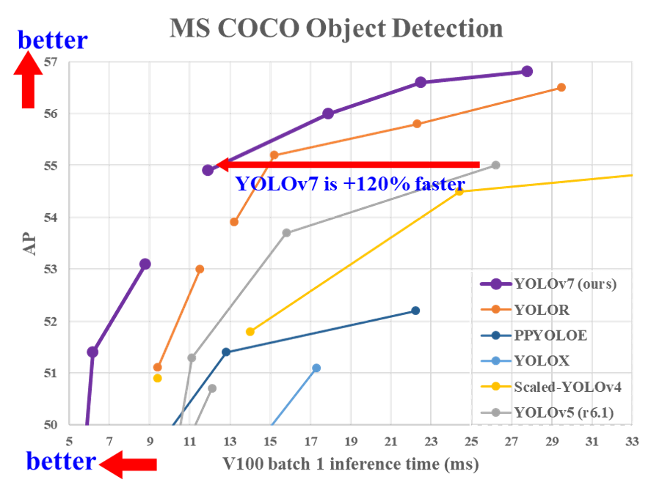
\includegraphics[width=0.4\textwidth]{images/Picture2.png}
    \caption{YOLOv7 comparison with other real-time object detectors. \cite{b6}}
    \label{fig:Picture2}
\end{figure}

Figure \ref{fig:Picture2} displays the performance of the YOLOv7 models compared to other object detection methods. The comparison is made by evaluating the inference time and Average Precision (AP) results. YOLOv7 performs 120\verb|%| faster and with better AP results \cite{b6}.

Aggarwal and Munjal \cite{b7} presents a method of using template matching to recognize the characters of the license plate. Their method includes preparing a database of templates using Microsoft paint, then after image preprocessing and character segmentation the character is matched with every template to identify the best match. Chen et al. \cite{b8} proposed using OpenCV’s image processing functions to identify the license plate and a 17-layer CNN model to recognize Chinese license plates. Jung and Kim \cite{b9} presented a system for license plate recognition that utilizes OpenCV’s image processing functionality as well and uses the Tesseract OCR (Optical Character Recognition) library, which is an OCR engine that supports character recognition in over 60 languages.  Optical Character Recognition (OCR) is a technology that takes an image containing text and outputs the text from the input, which can later be used for editing and searching. OCR uses machine learning algorithms to recognize and extract text from images. An image file goes through preprocessing, character segmentation and recognition, and other processes when OCR is applied \cite{b10}. 


\section{Plate Detection}

The first step in an ANPR system is plate detection. As mentioned in the literature review section of this paper there are a number of ways to localize an object from an image. The object detection algorithm used in this project is YOLOv7, the 7th version of YOLO which Wang et al. \cite{b6} developed. YOLO allows real-time object detection using convolutional neural networks (CNNs) to take input images and detect objects in them and it can identify a wide range of objects and outputs fast results with high accuracy. 

The YOLO algorithm works by separating an image into segments by placing a grid on top of an input image, as displayed in Figure \ref{fig:combined11} (a), and performing localization within each box of the grid \cite{b24}.  

Each detected object is assigned a confidence degree, which can be seen in Figure \ref{fig:combined11} (b). The thicker bounding boxes have a higher confidence than the thin ones \cite{b24}. 


\begin{figure}[ht]
  \centering
  \begin{subfigure}[b]{0.45\linewidth}
    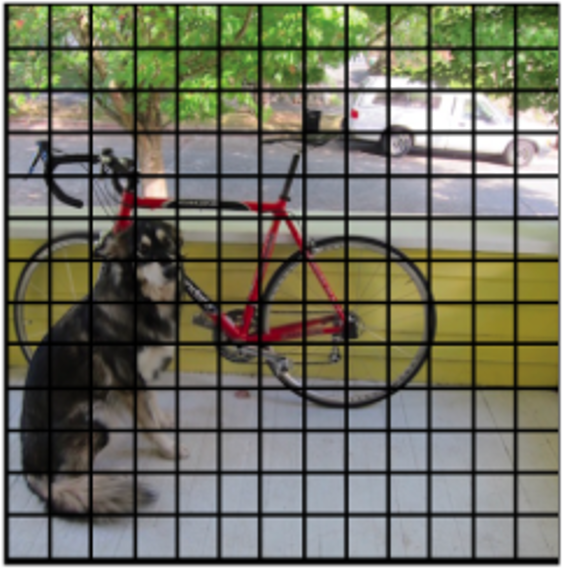
\includegraphics[width=\linewidth]{images/Picture34.png}
    \caption{Image after grid segmentation}
  \end{subfigure}
  \begin{subfigure}[b]{0.45\linewidth}
    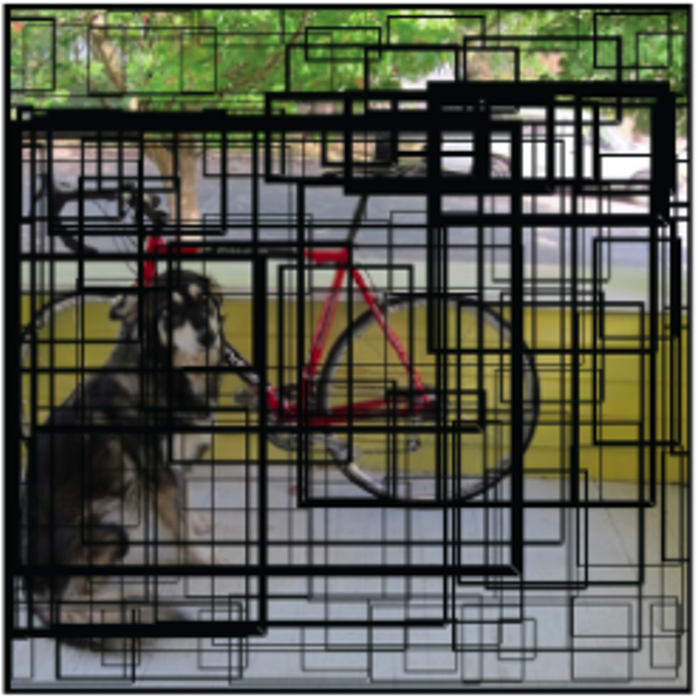
\includegraphics[width=\linewidth]{images/Picture35.png}
    \caption{Image after object localization}
  \end{subfigure}
  \caption{Object detected image and image after low confidence detection elimination}
  \label{fig:combined11}
  \cite{b24}
\end{figure}

After object localization, YOLO performs object classification by assigning each detected object a class. Based on the classification, all of the possible classes are highlighted and presented in Figure \ref{fig:combined10} (a). However, in order to increase accuracy and eliminate uncertainty, a confidence threshold is determined, which is 0.25 at default, and any classification with a confidence less than 0.25 is eliminated, leaving only the high-confidence objects depicted in \ref{fig:combined10} (b) \cite{b24}. 

\begin{figure}[ht]
  \centering
  \begin{subfigure}[b]{0.45\linewidth}
    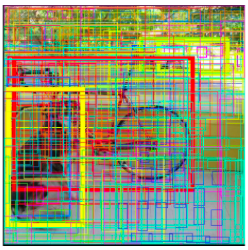
\includegraphics[width=\linewidth]{images/Picture37.png}
    \caption{Image with many low confidence objects detected}
  \end{subfigure}
  \begin{subfigure}[b]{0.45\linewidth}
    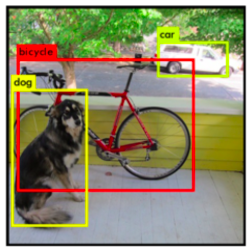
\includegraphics[width=\linewidth]{images/Picture38.png}
    \caption{Image after object low confidence boxes are removed}
  \end{subfigure}
  \caption{Object detected image and image after low confidence detection elimination}
  \label{fig:combined10}
\end{figure}

To train YOLOv7 to detect license plates, a dataset of images and their corresponding .txt files mentioned in the Data section that contain the coordinates of their license plate bounding box are necessary. Although YOLO can also be run on the CPU, it would take considerably longer to train, so for this project, Google Colab's GPU capabilities were used to train the model. The data was split to training and testing. Out of the total 170 images, 80\verb|%| were put in the training folder and the rest were used to test on. YOLOv7 takes this data and starts to train it. Initially, the data was used to train in batches of 16 images, repeated for 200 epochs. Once the algorithm has completed the training, a file “best.pt” is saved down which contains the weights with the best performance. An additional 100 epochs were required to train the model for satisfactory results. Following the completion of the training phase, YOLO was used to test the algorithm’s ability to identify license plates, and the results were saved to a designated folder. Figure \ref{fig:combined} (a) shows the input image and Figure \ref{fig:combined} (b) displays the results after YOLOv7’s inference was applied. YOLOv7 was successful and accurately identified the license plate in the provided image. The bounding box outputs the confidence of the algorithm which for Figure \ref{fig:combined} is 0.8. The inference script has a default confidence threshold value of 0.25, which specifies to the algorithm that if the confidence of the detected bounding box is less than 0.25 the bounding box will not be shown on the image. The algorithm also provided the precise coordinates of each detected license plate, which were later utilized for image preprocessing and character recognition purposes.

\begin{figure}[ht]
  \centering
  \begin{subfigure}[b]{0.45\linewidth}
    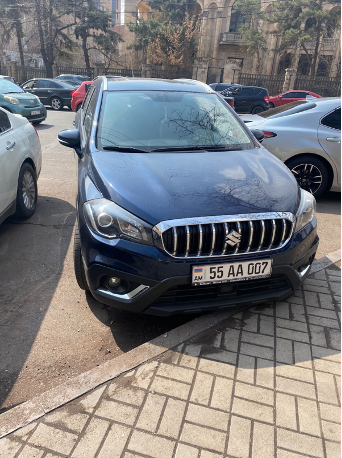
\includegraphics[width=\linewidth]{images/Picture3.png}
    \caption{Original Image from Dataset}
  \end{subfigure}
  \begin{subfigure}[b]{0.45\linewidth}
    \includegraphics[width=\linewidth]{images/Picture4.jpeg}
    \caption{Image after plate localization}
  \end{subfigure}
  \caption{Original Image and the image after YOLOv7 object detection was applied}
  \label{fig:combined}
\end{figure}

\section{Skew Adjustment}

One of ANPR's main challenges is identifying the orientation of the license plate and correcting the rotation. Many of the images in the dataset are taken at different angles which results in the license plates in the pictures being slightly rotated. If the orientation is not corrected the following character recognition procedures may not perform as well as they do on aligned license plate images. Multiple steps are involved to fix the orientation of the license plate, such as converting the image to grayscale, applying Canny edge detection \cite{b14} to identify the edges of the license plate, and using the Hough transform \cite{b15}, which detects and extracts straight lines in an image, and Affine transformation \cite{b17}, which preserves the shape of the input picture while changing the orientation. This chapter focuses on clarifying how these processing techniques work in adjusting the rotation of a license plate image. To adjust skew, an image needs to be cropped using the coordinates of the detected bounding box to only include the image of the license plate. 

\subsection{Grayscale}

Grayscaling is a process of transforming an image from having color into an image consisting of shades of gray. An example of a license plate image and its corresponding grayscale image are available in Figure \ref{fig:combine2}.  The grayscaling technique provides several benefits for image processing applications. Using gray images rather than color pictures is simple and easier to work with. A color image contains three color channels, one for each red, green, and blue component, whereas a gray image only has one color channel, making it less complex. It is also necessary to use grayscaling for image processing algorithms, such as the Canny edge detection function, which is designed to work specifically with grayscale images. By converting the image to grayscale, these algorithms can more easily detect and analyze the edges and shapes in the picture \cite{b11}. 

\begin{figure}[ht]
  \centering
  \begin{subfigure}[b]{0.45\linewidth}
    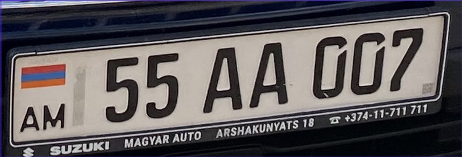
\includegraphics[width=\linewidth]{images/Picture5.png}
    \caption{Original image after cropping detected license plate}
  \end{subfigure}
  \begin{subfigure}[b]{0.45\linewidth}
    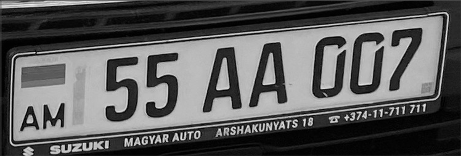
\includegraphics[width=\linewidth]{images/Picture6.png}
    \caption{Image after grayscale was applied}
  \end{subfigure}
  \caption{Visualization of cropped license plate image and the  grayscale image}
  \label{fig:combine2}
\end{figure}

\subsection{Canny Edge Detection}

Canny edge detection is one of the techniques implemented to fix the orientation of license plate images. As the name suggests, it is an algorithm for detecting the edges in a photo. Edge detection makes it simpler to recognize the characters on the plate. The edges allow for obtaining the boundaries and ultimate shape of the license plate. To give a better understanding of the outcome of edge detection, Figure \ref{fig:combined5} displays the result of canny edge detection applied to a number plate photo. 

\subsubsection{Gaussian Filter}

When canny edge detection is applied to an image, the image is first smoothed with a Gaussian filter, which is a 2D convolution kernel used to blur and reduce the noise in the image. Gaussian filters are applied to photos to make it easier for the edges to be identified \cite{b12}. 
The formula for applying the Gaussian filter is given by \ref{eq:gaussian-filter}:

\begin{equation}
G(x, y) = \frac{1}{2\pi\sigma^2} e^{-\frac{x^2+y^2}{2\sigma^2}}
\label{eq:gaussian-filter}
\end{equation}

The $x$ and $y$ values are the coordinates of a pixel being filtered. The $\sigma$ value is the standard deviation of the Gaussian kernel. \cite{b12}.

\subsubsection{Sobel Operator}

An edge in an image is the sudden change in the intensity of pixels, as shown in Figure \ref{fig:Picture7}. To detect edges in an image, the Sobel operator is utilized \cite{b12}.

\begin{figure}[h]
    \centering
    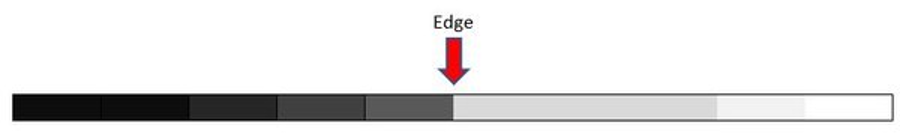
\includegraphics[width=0.4\textwidth]{images/Picture7.png}
    \caption{Visualization of an edge depicted by pixels \cite{b12}}
    \label{fig:Picture7}
    
\end{figure}

The algorithm involves using two 3x3 kernels shown in Figure \ref{fig:combined3}, which are another name for small matrices: the horizontal kernel, which calculates the intensity change of pixels in the horizontal direction (x-direction), and the vertical kernel, which calculates the intensity in the vertical direction (y-direction) \cite{b12}.

\begin{figure}[ht]
  \centering
  \begin{subfigure}[b]{0.45\linewidth}
    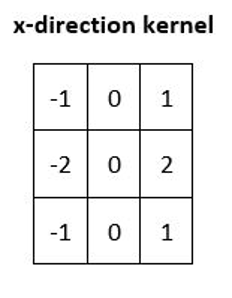
\includegraphics[width=\linewidth]{images/Picture8.png}
    \caption{Horizontal Direction Kernel}
  \end{subfigure}
  \begin{subfigure}[b]{0.45\linewidth}
    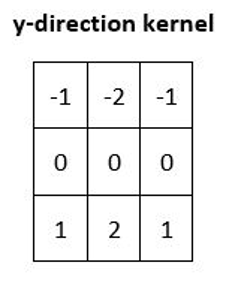
\includegraphics[width=\linewidth]{images/Picture9.png}
    \caption{Verticle Direction Kernel}
  \end{subfigure}
  \caption{The Sobel kernels in the horizontal and vertical directions \cite{b12}}
  \label{fig:combined3}
  
\end{figure}

To understand a pixel's intensity and the change of intensity, the gradient is calculated, which is the derivative of a given pixel \cite{b12}.  

\begin{equation}
    G_x = \begin{bmatrix}
    -1 & 0 & 1 \\
    -2 & 0 & 2 \\
    -1 & 0 & 1
    \end{bmatrix} * A(x, y)
    \label{eq:GX}
\end{equation}

\begin{equation}
    G_y = \begin{bmatrix}
    -1 & -2 & -1 \\
    0 & 0 & 0 \\
    1 & 2 & 1
    \end{bmatrix} * A(x, y)
    \label{eq:GY}
\end{equation}

The formulas \ref{eq:GX} and \ref{eq:GY} calculate the gradient in the x and y directions, where $*$ is a convolution operation, the calculation will be explained further on in the paper, and $A(x, y)$ is the 3x3 portion of image A with $(x,y)$ as the center cell \cite{b12}. 

\begin{equation}
    G = \sqrt{G_x^2 + G_y^2}
    \label{eq:magnitude}
\end{equation}

\begin{equation}
    \theta = \arctan(G_y/G_x)
    \label{eq:gradient}
\end{equation}

Once the Gx and Gy are calculated, the magnitude $(G)$ of the gradient at pixel $(x,y)$ and the direction of the gradient ($\theta$) can be calculated by the formulas \ref{eq:magnitude} and \ref{eq:gradient} \cite{b12}.

\begin{figure}[h]
    \centering
    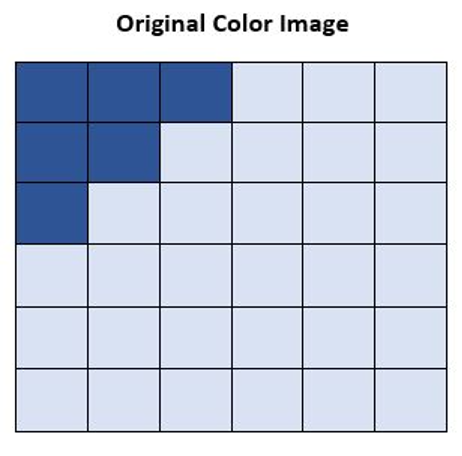
\includegraphics[width=0.3\textwidth]{images/Picture10.png}
    \caption{Color image with edge \cite{b12}}
    \label{fig:Picture10}
    
\end{figure}

To best understand how the Sobel operator works, an example calculation is done on Figure \ref{fig:Picture10}. At first glance at Figure \ref{fig:Picture10}, it is evident that the image changes in intensity. The first step to detect the edge of the pixels is to convert the image to grayscale, which is displayed in Figure \ref{fig:Picture11} \cite{b12}.

\begin{figure}[h]
    \centering
    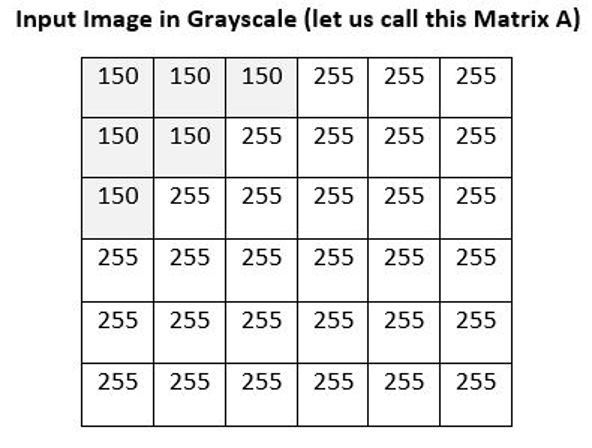
\includegraphics[width=0.3\textwidth]{images/Picture11.png}
    \caption{Grayscale image of Figure 7 with intensity values \cite{b12}}
    \label{fig:Picture11}
    
\end{figure}

To calculate the gradients $G_x$ and $G_y$ of the pixel in the second row and column, Figure \ref{fig:Picture11} needs to be convolved with the $x$ and $y$ directional kernels depicted in Figure \ref{fig:combined3} by first calculating the gradient in the vertical direction ($G_y$). The y-direction kernel is overlaid on Figure \ref{fig:Picture11}, resulting in the visualization in Figure \ref{fig:Picture12}. Next, the x-direction kernel is overlaid onto Figure \ref{fig:Picture11} \cite{b12}. 

\begin{figure}[h]
    \centering
    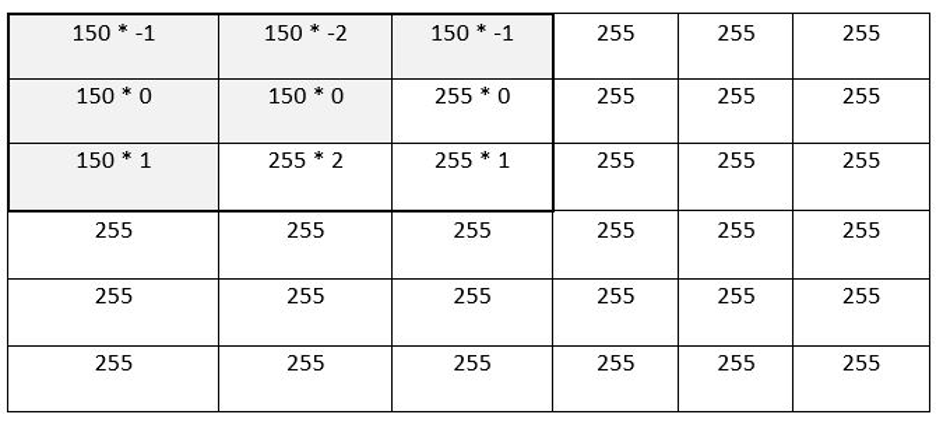
\includegraphics[width=0.4\textwidth]{images/Picture12.png}
    \caption{The y-direction kernel overlaid on a grayscale image with intensity values displayed \cite{b12}}
    \label{fig:Picture12}
    
\end{figure}

The intensity values in Figure \ref{fig:Picture12} are multiplied by the x and y-direction kernel values, which result in Figure \ref{fig:combined4} \cite{b12}. 

\begin{figure}[ht]
  \centering
  \begin{subfigure}[b]{0.45\linewidth}
    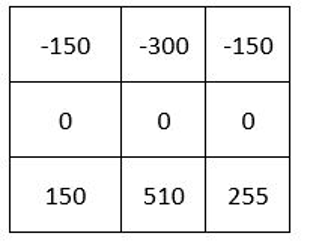
\includegraphics[width=\linewidth]{images/Picture13.png}
    \caption{y-direction kernel}
  \end{subfigure}
  \begin{subfigure}[b]{0.45\linewidth}
    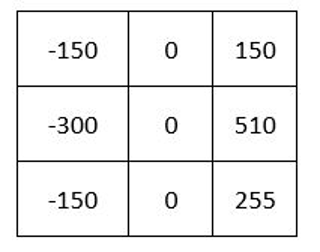
\includegraphics[width=\linewidth]{images/Picture14.png}
    \caption{x-direction kernel}
  \end{subfigure}
  \caption{Resulting values of horizontal and vertical kernel multiplication to a portion of pixels \cite{b12}}
  \label{fig:combined4}
  
\end{figure}

The values of each resulting direction are added, and the $G_x$ and $G_y$ value for the pixel in row and column two is 315. The magnitude is $\approx$ 445. This calculation is done for each pixel, and the highest magnitudes are considered the edges \cite{b12}.

\subsubsection{Non-maximum Suppression and Hysteresis Thresholding}

Non-maximum suppression clears the image by removing unnecessary lines and keeping only the highest points in the gradient. It compares each pixel's gradient strength to the strengths of its two neighboring pixels in the direction of the gradient. If a pixel's strength is higher than its neighbors, it is marked as a "local maximum"; if not, it is suppressed \cite{b13}. 

\begin{figure}[h]
    \centering
    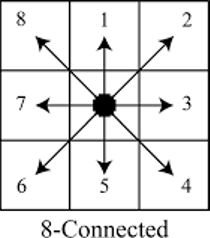
\includegraphics[width=0.1\textwidth]{images/Picture15.png}
    \caption{Visualization of 8-connectivity neighborhood \cite{b13}}
    \label{fig:Picture15}
    
\end{figure}

Hysteresis thresholding connects the strong edges and represses the weak edges of a given image. This is done by assigning threshold values for a high and low threshold. Then, the pixels are filtered to check their gradient magnitude and compare them with the threshold values. If the pixel's gradient magnitude exceeds the high threshold value, it is considered a strong edge. If the gradient magnitude is lower than the low threshold, it is considered a weak edge. When a pixel's gradient magnitude is between the two threshold values, it is considered a part of an edge if they are connected to a strong edge. Otherwise, it is a weak edge. A weak and strong edge are connected if the weak edge is one of the eight neighbors of the strong edge, otherwise known as 8-connectivity shown in Figure \ref{fig:Picture15}. The resulting output is a binary image where the strong edges are marked as white pixels, and the weak edges are black pixels \cite{b13}.

\begin{figure}[ht]
  \centering
  \begin{subfigure}[b]{0.45\linewidth}
    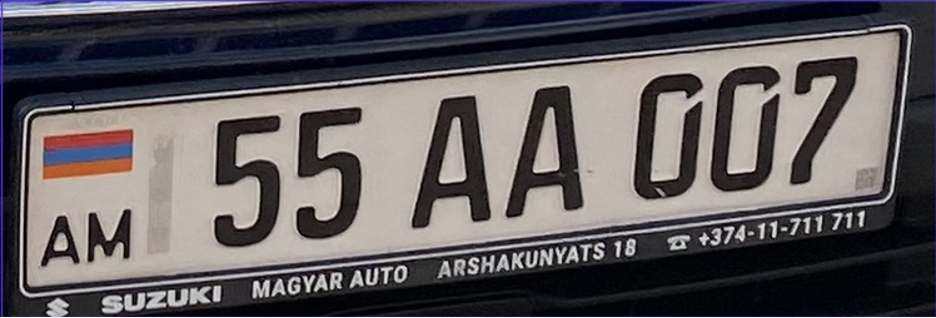
\includegraphics[width=\linewidth]{images/Picture16.png}
    \caption{Original image after cropping detected license plate. }
  \end{subfigure}
  \begin{subfigure}[b]{0.45\linewidth}
    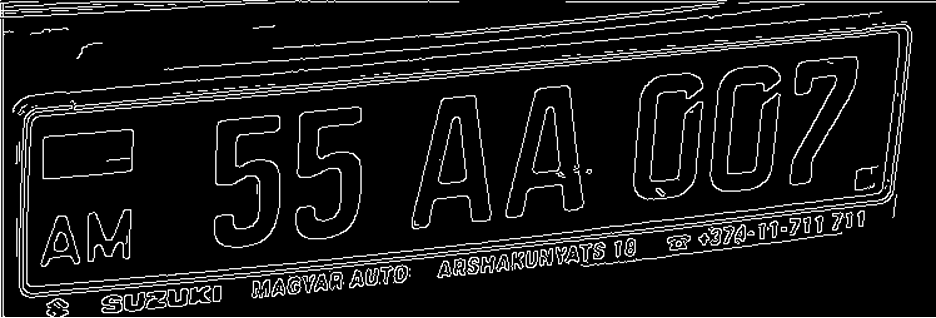
\includegraphics[width=\linewidth]{images/Picture17.png}
    \caption{Image after edge detection is applied}
  \end{subfigure}
  \caption{Cropped License Plate Image and Edge Detected Image}
  \label{fig:combined5}
\end{figure}

To conclude, the Canny edge detection algorithm works by smoothing an image and calculating the gradient magnitude and gradient orientation for each pixel of the image. The image goes through non-maximum suppression, and finally, hysteresis thresholding is applied. The license plate image after canny edge detection has been used is depicted in Figure \ref{fig:combined5}. Please see \cite{b14} for details.

\subsection{Hough Transform}

The next step in ANPR is applying Hough transform to an image, which is another image processing algorithm that detects and extracts straight lines in an image. This part of the process is necessary for locating the orientation of the characters on a license plate. 
Representing a straight line using two parameters, slope, and intercept, denoted by $(a,b)$, is a well-known concept in elementary mathematics and is given by Formula \ref{eq:line} \cite{b15}.

\begin{equation}
    y = ax + b
    \label{eq:line}
\end{equation}

However, an alternative approach to uniquely defining a line is by utilizing the polar system, involving two parameters $(\rho, \theta)$, depicted in Figure \ref{fig:Picture18}. $\rho$ refers to the perpendicular distance from the origin to the line, $\theta$ represents the angle between the x-axis and the distance line. This polar representation enables the description of vertical lines, which is not feasible using the $(a,b)$ parameters in the Cartesian system \cite{b15}.

\begin{figure}[h]
    \centering
    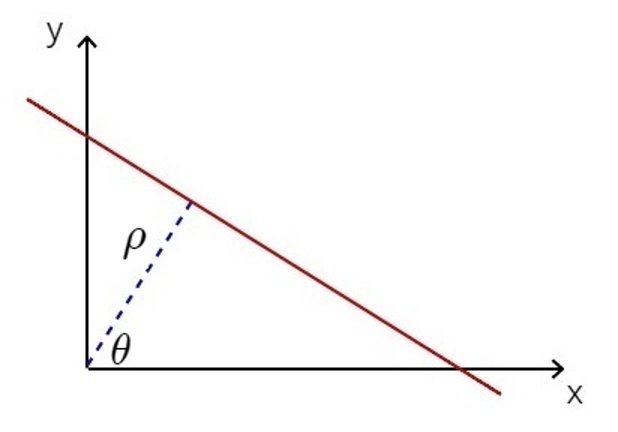
\includegraphics[width=0.3\textwidth]{images/Picture18.png}
    \caption{The $\rho$, $\theta$ parameters in the Cartesian Coordinate System \cite{b15}}
    \label{fig:Picture18}
    
\end{figure}

The formula for converting a line from the Cartesian coordinate system to a point in the polar coordinate system is given by the following formula:

\begin{equation}
    \rho = x \cos\theta + y \sin\theta
    \label{eq:polar}
\end{equation}

These $(\rho, \theta)$ coordinates can be plotted in the Hough space, which denotes the set of all lines that pass through a specific point in the image space.

\begin{figure}[h]
    \centering
    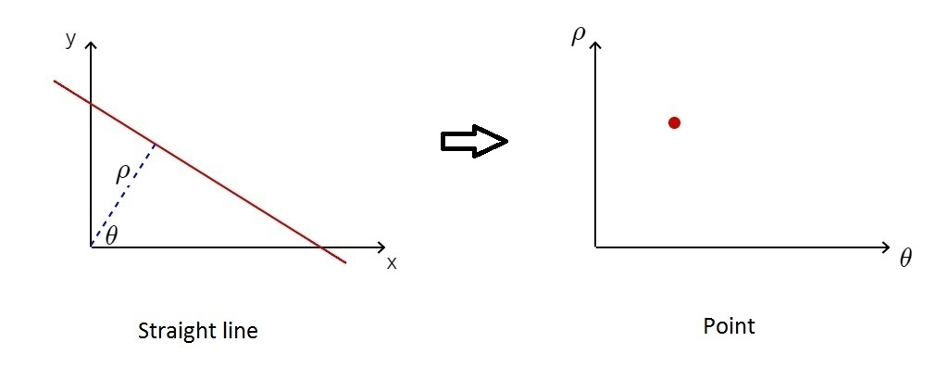
\includegraphics[width=0.4\textwidth]{images/Picture19.png}
    \caption{Visualization  of a line represented in the Hough space by the ($\rho, \theta$) parameters \cite{b15}}
    \label{fig:Picture19}
    
\end{figure}

A line in the Cartesian coordinate system is equivalent to a point in the Hough space, which denotes the set of all lines that pass through a specific point in the image space. This is displayed in Figure \ref{fig:Picture19}. When several lines are drawn in the image space that intersect at one point, they correspond to a sinusoid in the Hough space, as shown in Figures \ref{fig:Picture20}. Plotting multiple lines in the image space leads to several sinusoids in the Hough space that intersect at a common point. The intersection point represents the straight lines and intersections in the Hough space can be searched to identify them. These intersections correspond to the straight lines' representative ($\rho, \theta$) parameters \cite{b15}. 

\begin{figure}[h]
    \centering
    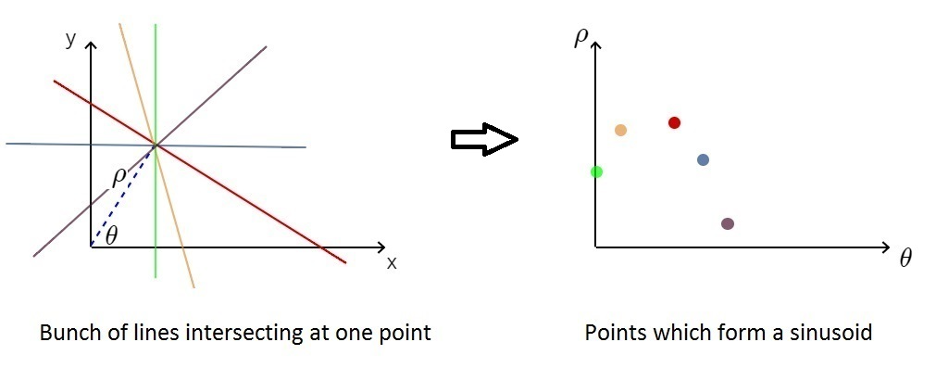
\includegraphics[width=0.4\textwidth]{images/Picture20.png}
    \caption{Representation of many intersecting lines in the image and Hough spaces \cite{b15}}
    \label{fig:Picture20}
    
\end{figure}

The point where the sinusoids intersect in the Hough space shows where the straight lines are located in the image space. These straight lines can be found by looking for these intersection points in the Hough space. Therefore, if a point is drawn in the image space, the result in the Hough space will be a sinusoid, as displayed in Figure \ref{fig:Picture21}. The ($\rho, \theta$) values of these intersection points represent the parameters of the straight lines \cite{b15}. 

\begin{figure}[h]
    \centering
    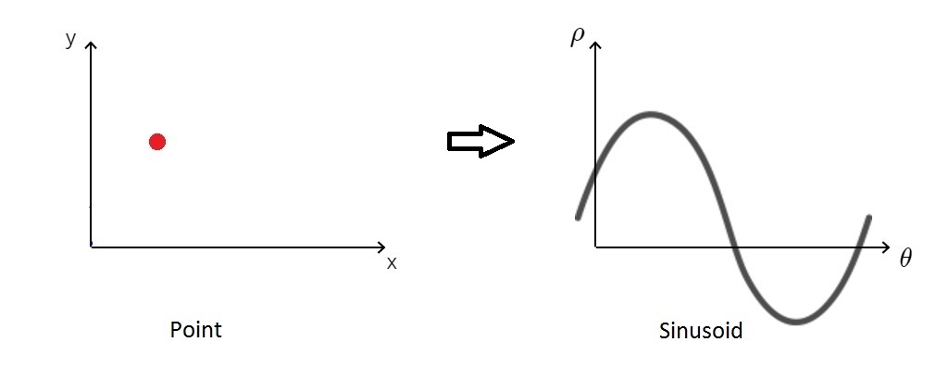
\includegraphics[width=0.4\textwidth]{images/Picture21.png}
    \caption{Visualization of a point in the image space corresponding to a sinusoid in the Hough Space \cite{b15}}
    \label{fig:Picture21}
    
\end{figure}

When points that form a line in the image space are plotted, they give rise to a set of sinusoids in the Hough space, depicted in Figure \ref{fig:Picture22}. Remarkably, the sinusoids generated from these points intersect at precisely one point. This property enables the Hough transform to identify straight lines in an image. The intersection point in the Hough space represents the parameters of the straight line in the image space \cite{b15}. 

\begin{figure}[h]
    \centering
    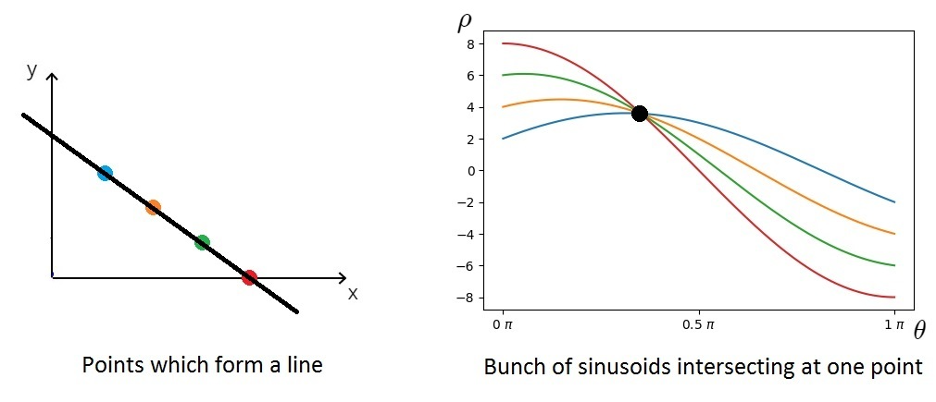
\includegraphics[width=0.4\textwidth]{images/Picture22.png}
    \caption{Representation of points forming a line in the image and Hough Spaces \cite{b15}}
    \label{fig:Picture22}
    
\end{figure}

By applying this technique to an image of a license plate, in Figure \ref{fig:combined6}, the implementation of a Hough transform applied to an image of a  license plate can be observed. 

\begin{figure}[ht]
  \centering
  \begin{subfigure}[b]{0.45\linewidth}
    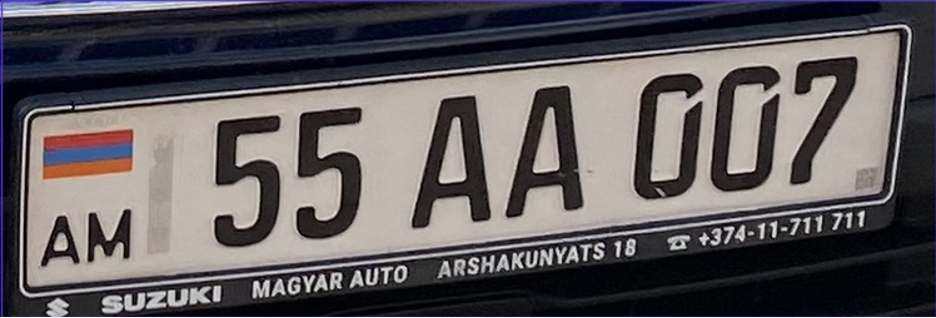
\includegraphics[width=\linewidth]{images/Picture23.png}
    \caption{Original image after cropping detected license plate}
  \end{subfigure}
  \begin{subfigure}[b]{0.45\linewidth}
    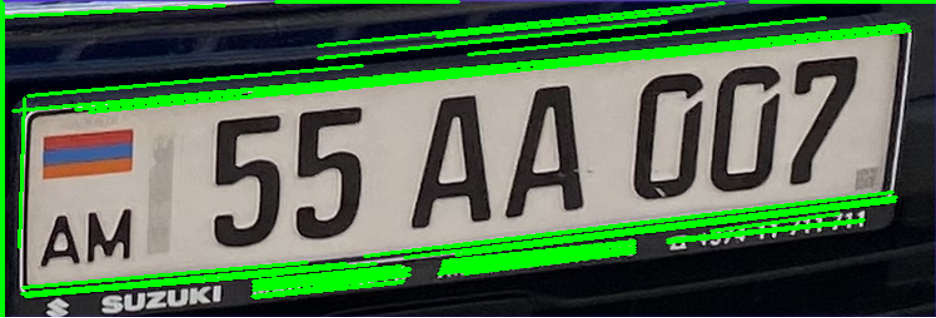
\includegraphics[width=\linewidth]{images/Picture24.png}
    \caption{Image after Lines Detected using Hough Transform}
  \end{subfigure}
  \caption{Cropped License Plate Image and Image after Hough Transform}
  \label{fig:combined6}
\end{figure}

\subsection{Rotation Angle Calculation}

After Hough Transform has been implemented, the lines detected can be used to calculate the rotation of the angle. To calculate the angle between a line and the x-axis, the coordinates for two points: $(x_1, y_1)$ and $(x_2, y_2)$, which connect the line on the image, are taken. The formula \ref{eq:angle} is used to calculate the angle ($\alpha$). 

\begin{equation}
    \alpha = \arctan\left(\frac{y_2-y_1}{x_2-x_1}\right) * \frac{180}{\pi}
    \label{eq:angle}
\end{equation}

For each line, the angle is calculated then the median angle is selected as the rotation angle.

\subsection{Affine Transformation with Rotation Matrix}

Once the dominant angle has been selected, a rotation matrix is computed. To compute a rotation matrix, M the \texttt{getRotationMatrix2D} function is used, which inputs the center point, rotation angle, and a scale factor of 1.0. The function for computing the rotation matrix M can be observed in Formula \ref{eq:matrix}, where, $\alpha = scale \cdot \cos{\theta}$, $\beta = scale \cdot \sin{\theta}$, and $C_x$ and $C_y$ are the coordinates of the center of the image. It returns a 2x3 affine transformation matrix that can be used to rotate and scale the image \cite{b16}.  

\begin{equation}
    M = \begin{bmatrix}
        \alpha & \beta & (1-\alpha) \cdot C_x - \beta \cdot C_y\\
        -\beta & \alpha & \beta \cdot C_x + (1-\alpha) \cdot C_y
    \end{bmatrix}
    \label{eq:matrix}
\end{equation}

The next step is to apply the rotation matrix M to the input image using an Affine transformation. An Affine transformation is a 2D linear transformation that preserves the straightness of lines by taking the source image, the M rotation matrix, and the size of the output image and producing a straightened image. The transformation is widely used in image processing for correcting the orientation of images. For this project, by applying the Affine transformation, the license plate image skew is adjusted as seen in Figure \ref{fig:combined7}, resulting in higher character recognition accuracy. For more details about affine transformations please see \cite{b17}.

\begin{figure}[ht]
  \centering
  \begin{subfigure}[b]{0.45\linewidth}
    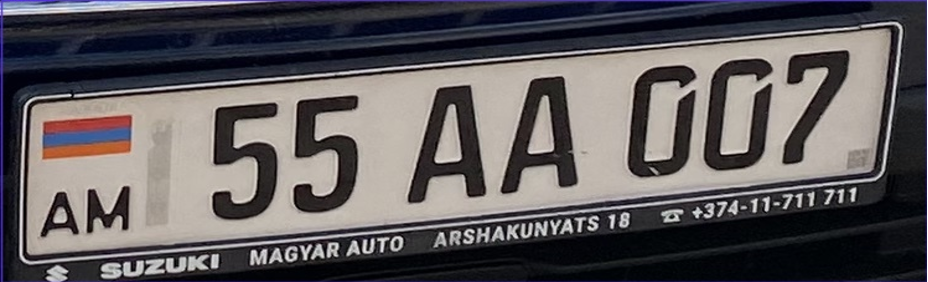
\includegraphics[width=\linewidth]{images/Picture26.png}
    \caption{Original image after cropping detected license plate}
  \end{subfigure}
  \begin{subfigure}[b]{0.45\linewidth}
    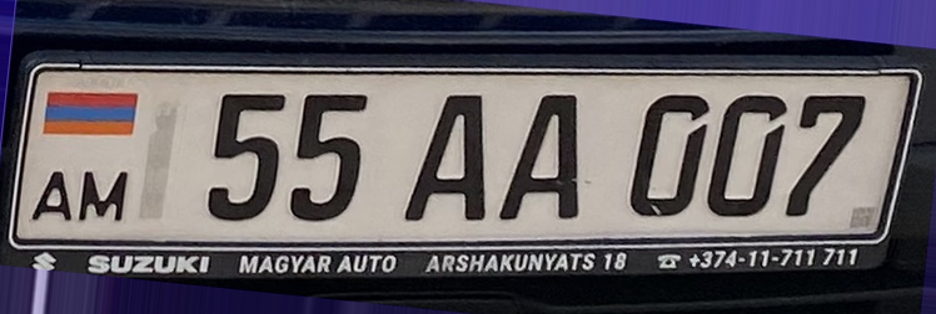
\includegraphics[width=\linewidth]{images/Picture27.png}
    \caption{Image after the Orientation Correction}
  \end{subfigure}
  \caption{Cropped License Plate Image and Rotation Adjusted Image}
  \label{fig:combined7}
\end{figure}

\section{Character Recognition}
\subsection{Contour Detection and Aspect Ratio}

Contour detection is the primary technique used in image processing, and it can often be used to localize and separate multiple objects in a given image. Contour detection has played a massive role in numerous applications such as image segmentation, object recognition, etc. A contour is a curve that connects the points of similar intensity and color on the boundary of an object. In order to detect and visualize the contours in OpenCV, two functions are utilized: the \texttt{findContours()} function, which detects the contours of the license plates in the image, and the \texttt{drawContours()} function, which overlays the identified contours on the original image \cite{b18}.

In the context of this project, contour detection is helpful for accurately identifying the characters' boundaries in the license plate, as demonstrated in Figure \ref{fig:combined8}. The algorithm successfully separated the characters' contours and the license plate itself. To identify the contour of the license plate, it is necessary to check the aspect ratio of each contour and check if the ratio matches the ratio of a license plate \cite{b19}.

The aspect ratio formula is given by Formula \ref{eq:ratio}.

\begin{equation}
    ratio = \frac{width}{height}
    \label{eq:ratio}
\end{equation}

\begin{figure}[ht]
  \centering
  \begin{subfigure}[b]{0.45\linewidth}
    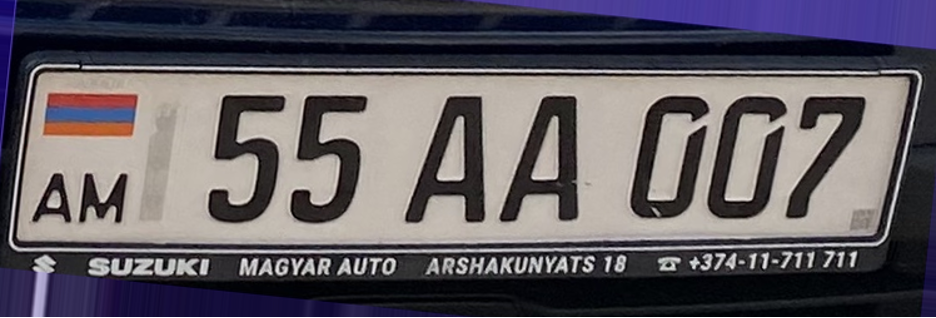
\includegraphics[width=\linewidth]{images/Picture28.png}
    \caption{Skew adjusted image}
  \end{subfigure}
  \begin{subfigure}[b]{0.45\linewidth}
    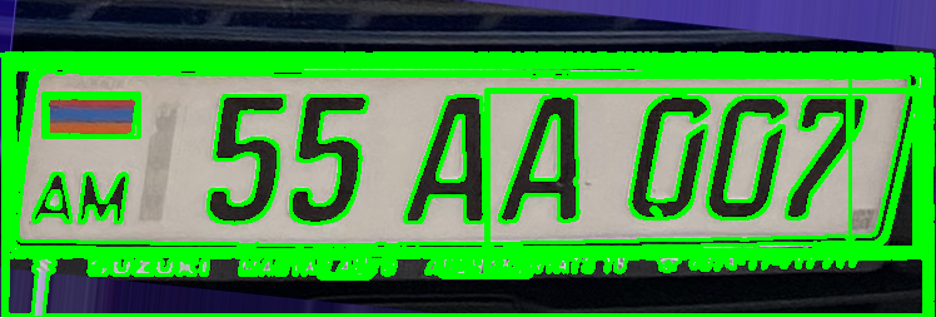
\includegraphics[width=\linewidth]{images/Picture29.png}
    \caption{Detected contours on image}
  \end{subfigure}
  \caption{ Rotated Image and Contours Detected Image}
  \label{fig:combined8}
\end{figure}

\subsection{EasyOCR}

Once the license plate has been detected and the orientation of the plate has been adjusted, the next step in this ANPR project is character recognition. For this implementation, EasyOCR was utilized to obtain the license plate text. EasyOCR is a Python library that simplifies Optical Character Recognition (OCR) for computer vision developers. As its name suggests, it is easy to use and is considered the most uncomplicated method for applying OCR \cite{b20}.
Due to its easy integration of OCR and high accuracy results, applying EasyOCR directly without the use of additional CNN training was a simple approach to get high results.

\begin{figure}[ht]
  \centering
  \begin{subfigure}[b]{0.45\linewidth}
    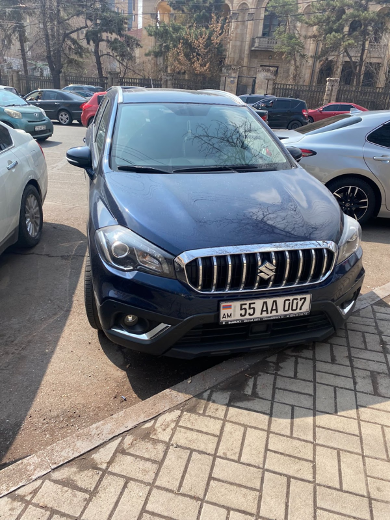
\includegraphics[width=\linewidth]{images/Picture30.png}
    \caption{Original Image}
  \end{subfigure}
  \begin{subfigure}[b]{0.45\linewidth}
    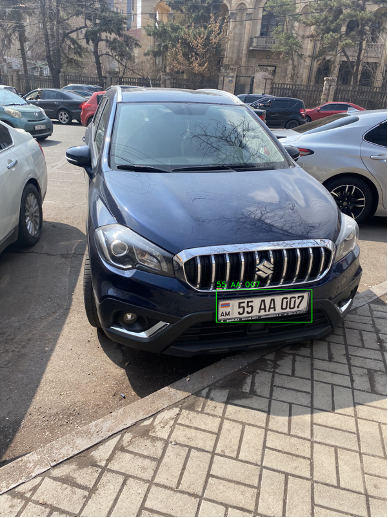
\includegraphics[width=\linewidth]{images/Picture31.png}
    \caption{Image after ANPR}
  \end{subfigure}
  \caption{Original Image and Image after Automated Number Plate Recognition}
  \label{fig:combined9}
\end{figure}

The result of the ANPR system applied to an image is shown in Figure \ref{fig:combined9}. 

\section{Detection and Recognition on Videos}

Although the main aspects of ANPR remain the same when applying it to videos, some additional steps must be taken. Initially, YOLOv7 is used to detect the license plates from the video and output a video with the detected license plates and their corresponding bounding box coordinate files. YOLOv7 splits the video into frames, applies object detection on each frame, and saves the coordinates of the bounding box of each frame.  

The next step is to split the video into frames; the frames are then cropped to include only the license plate, preprocessing is applied to the cropped frame, the orientation of the plate is adjusted, and EasyOCR is applied to recognize the text. Next, the bounding box coordinates are used to draw a bounding box around the detected frame and add the recognized text. The resulting image is similar to Figure \ref{fig:combined9} and is saved in a separate folder. Once all of the video frames have undergone this process, OpenCV's video processing functions are used to add all of the frames together and output the video file. An example of a detected video can be found in the GitHub repository of this project. 


To reduce computation time of video processing, instead of processing each frame per second (which could be around 30 frames per second), every 5th frame was processed. The smoothness of the video was reduced but the computation time is saved by a factor of 5. 
For instance, if the original video was 10 seconds long and had 300 frames (30 frames per second), only 60 frames would be processed. However, if these 60 frames were written into a video with the default frame rate of 30 frames per second, the resulting video would only be 2 seconds long (60/30).

To avoid this issue and maintain the original length and speed of the video, the output video frame rate was adjusted to 6 frames per second. This compensates for the fact that the original video was being reduced by a factor of 5, meaning that each second of the original video is now represented by 1 second / 5 = 0.2 seconds in the new video. Therefore, the frame rate also needs to be reduced by a factor of 5 to maintain the original speed of the video.

\section{Results and Discussion}
\subsection{Plate Localization Results}

The results of the YOLOv7 object detection algorithm can be evaluated by multiple criteria such as precision, recall and mAP (mean Average Precision). 

\begin{figure}[h]
    \centering
    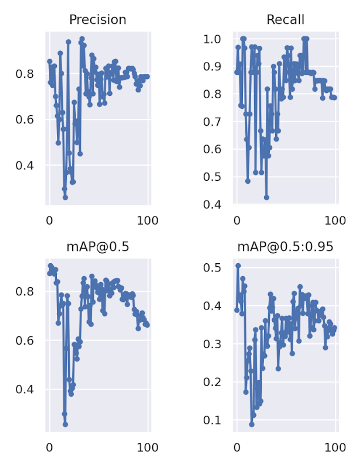
\includegraphics[width=0.3\textwidth]{images/Picture32.png}
    \caption{Plots of the precision, recall, and mAP of the training  of license plate detection in YOLOv7 }
    \label{fig:Picture32}
\end{figure}

The precision can be defined as how often the model detection is correct , and the recall can be described as a metric that evaluates if the model has detected the object each time it was present \cite{b2}.

The formulas to calculate the precision and recall are given by Formula \ref{eq:precision} and \ref{eq:recall}, where $TP$ is the number of true positive results, $FP$ is the number of false positive results, and $FN$ is the number false negative results.

\begin{equation}
    precision = \frac{TP}{TP + FP}
    \label{eq:precision}
\end{equation}

\begin{equation}
    recall = \frac{TP}{TP + FN}
    \label{eq:recall}
\end{equation}

The results of the training of YOLOv7 on the dataset with 100 epochs can be seen in Figure \ref{fig:Picture32}, which shows metrics such as precision and recall throughout the training. By the end of the training the precision is close to 80\verb|%| and the recall is between 80-90\verb|%|. After training object detection using YOLOv7, the algorithm is tested. As depicted in Figure \ref{fig:Picture33}, the training results were successful, and the algorithm could detect license plates accurately. 

\begin{figure}[h]
    \centering
    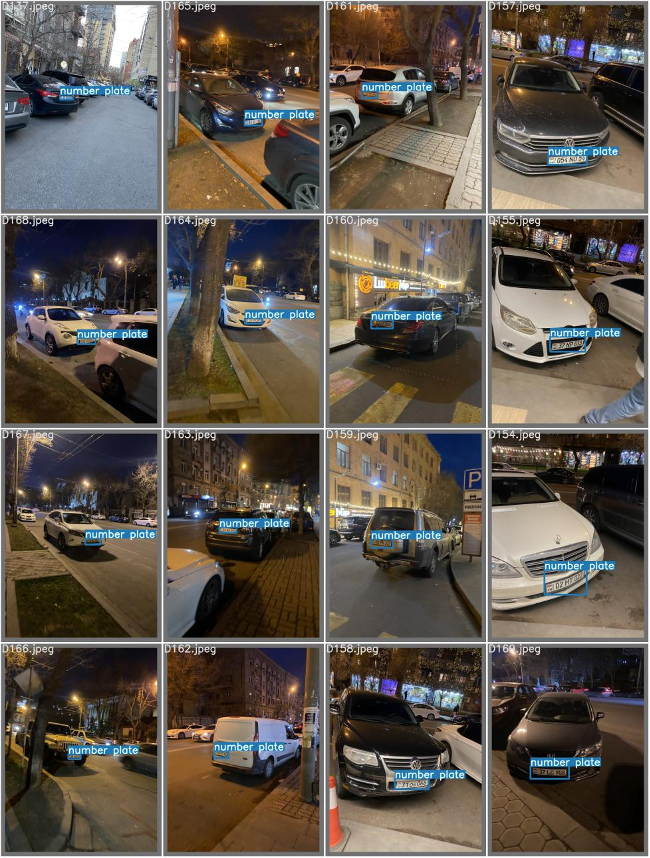
\includegraphics[width=0.5\textwidth]{images/Picture33.png}
    \caption{Results of test batch after training YOLO}
    \label{fig:Picture33}
\end{figure}

\subsection{Character Recognition Results}

To test the results of the EasyOCR implementation, a subset of the data used for training license plate detection was used to test the results. The label data of the images was used to crop the dataset into just the license plate pictures. Next, the data went through skew adjustment, and EasyOCR was applied. The algorithm's results were compared to a list containing the actual license plate numbers. 155 out of 161 characters were recognized correctly, giving an overall accuracy of 96\verb|%|. Another metric used to test the performance of the character recognition was the Levenshtein distance which compares two strings and outputs a number of how different they are\cite{b22}. 

The formula to compute the Levenshtein distance given two strings $a$ and $b$ is the following: 

\begin{equation}
lev_{\scriptstyle a,b}(i,j) =
\begin{cases}
    \max(i,j), \qquad \text{if} \min(i,j) = 0, \\
    \min\begin{cases} 
        lev_{\scriptstyle a,b}(i-1,j)+1, \\
        lev_{\scriptstyle a,b}(i,j-1)+1, \\
        lev_{\scriptstyle a,b}(i-1,j-1)+1_{\scriptstyle(a_i \neq b_j)}, & \text{otherwise}
    \end{cases}
\end{cases}
\label{eq:levenshtein}
\end{equation}

The $i$ and $j$ values refer to the character positions of strings $a$ and $b$ respectfully. The results showed the average distance between two strings to be 0.25 \cite{b22}. 

\section{Conclusion and Future Work}

This project has developed an Automatic Number Plate Recognition (ANPR) system to perform image processing and produce accurate results. The system implements object detection using the YOLOv7 object detection model, OpenCV’s library of functions for converting an image to grayscale, detecting the edges, identifying the straight lines, computing the angle by which the image lines are skewed, fixing the orientation of the license plate, and recognizing the license plate characters.  The system has achieved a high accuracy rate of 90\verb|%| on plate detection and 95\verb|%| on character recognition on a dataset consisting of Armenian license plates. Despite these promising results, there is still scope for improvement, and it is essential to evaluate the project objectively and identify areas for further development.

One of the major areas for improvement of the system is the computation time. Although it is able to detect and recognize license plate numbers on videos, the running time of the system is high. The project would benefit greatly from finding more optimal solutions to the problem.

Due to the scarcity of data available in Armenia, the dataset used in this project was manually collected by capturing images using a smartphone. This method has produced a dataset consisting mainly of high-quality photos and videos. However, to test the system's effectiveness, obtaining a dataset with lower-quality images and videos would be necessary. Although EasyOCR has delivered promising results with high-quality data, it would be worthwhile to explore the possibility of training a Convolutional Neural Network (CNN) to recognize low-quality characters in images.

To enhance this project, exploring additional data acquisition methods and the image processing techniques may be necessary. Additionally, it would be helpful to optimize the computational time cost of the system in order to provide more opportunities of application of the system.

%\section*{References}

\begin{thebibliography}{00}
\bibitem{b1} heartexlabs. (2022, September). labelImg. Github. \url{https://github.com/heartexlabs/labelImg}

\bibitem{b2} Kaur, S., Jain, A., Gupta, J., \& Khandelwal, S. (2021). Vehicle License Plate Recognition. Zenodo (CERN European Organization for Nuclear Research). \url{https://doi.org/10.5281/zenodo.5171216}

\bibitem{b3} Boesch, G. (2023). Object Detection in 2023: The Definitive Guide. viso.ai. 
\url{https://viso.ai/deep-learning/object-detection/#:~:text=on%20Viso%20Suite-,Most%20Popular%20Object%20Detection%20Algorithms,the%20single%2Dshot%20detector%20family.}

\bibitem{b4} Podorozhniak, A., Liubchenko, N., Sobol, M., \& Onishchenko, D. (2023). USAGE OF MASK R-CNN FOR AUTOMATIC LICENSE PLATE RECOGNITION. Sučasnì Ìnformacìjnì Sistemi, 7(1), 54–58. \url{https://doi.org/10.20998/2522-9052.2023.1.09}

\bibitem{b5} Awati, R. (2023). convolutional neural network (CNN). Enterprise AI. \url{https://www.techtarget.com/searchenterpriseai/definition/convolutional-neural-network}

\bibitem{b23} Grigoryan, M., \& Matinyan, A. (2020). Automatic Vehicle Number Plate Detection and Recognition. American University of Armenia


\bibitem{b6} Wang et al. (2022). YOLOv7: Trainable bag-of-freebies sets new state-of-the-art for real-time object detectors. arXiv preprint arXiv:2207.02696. 
\url{https://github.com/WongKinYiu/yolov7}

\bibitem{b7} Aggarwal, N., \& Munjal, S. (2022). Automated Number Plate Recognition Using Template Matching. www.academia.edu. \url{https://www.academia.edu/69856610/Automated_Number_Plate_Recognition_Using_Template_Matching}

\bibitem{b8} Chen, H., Lin, Y., \& Zhao, T. (2023). Chinese License Plate Recognition System Based on Convolutional Neural Network. Highlights in Science, Engineering and Technology, 34, 95–102. \url{https://doi.org/10.54097/hset.v34i.5386}

\bibitem{b9} Jung, Y. C., \& Kim, H. J. (2018). Design and implementation of lightweight vehicle license plate recognition module utilizing open CV and Tesseract OCR library. International Journal of Engineering \& Technology. \url{https://doi.org/10.14419/ijet.v7i2.33.14184}

\bibitem{b10} What is OCR? - Optical Character Recognition Explained - AWS. (n.d.). Amazon Web Services, Inc. \url{https://aws.amazon.com/what-is/ocr/#:~:text=Optical%20Character%20Recognition%20(OCR)%20is,scan\%20as%20an%20image%20file.}

\bibitem{b24} Yolov7: Artificial Intelligence for real-time object detection in an image. (2023, January 19). Novelis Innovation. 
\url{https://novelis.io/news/yolov7-artificial-intelligence-for-real-time-object-detection-in-an-image/}

\bibitem{b11} GeeksforGeeks. (2023). Python  Grayscaling of Images using OpenCV. GeeksforGeeks. 
\url{https://www.geeksforgeeks.org/python-grayscaling-of-images-using-opencv/}

\bibitem{b12} Sears-Collins, A. (2019, December). How the Sobel Operator Works. AutomaticAddison.com. \url{https://automaticaddison.com/how-the-sobel-operator-works/}

\bibitem{b13} He, Y., Hu, T., \& Zeng, D. (2019). Scan-flood Fill(SCAFF): an Efficient Automatic Precise Region Filling Algorithm for Complicated Regions. \url{https://www.researchgate.net/publication/333678982_Scan-flood_FillSCAFF_an_Efficient_Automatic_Precise_Region_Filling_Algorithm_for_Complicated_Regions}

\bibitem{b14} OpenCV: Canny Edge Detection. (n.d.). OpenCV. \url{https://docs.opencv.org/4.x/da/d22/tutorial_py_canny.html}

\bibitem{b15} Tomasz.Kacmajor. (2020, May 17). Hough Lines Transform Explained - tomaszkacmajor.pl. tomaszkacmajor.pl. 
\url{https://tomaszkacmajor.pl/index.php/2017/06/05/hough-lines-transform-explained/}

\bibitem{b16} GeeksforGeeks. (2023). OpenCV:  getRotationMatrix2D  Function. GeeksforGeeks. 
\url{https://www.geeksforgeeks.org/python-opencv-getrotationmatrix2d-function/}

\bibitem{b17} OpenCV: Affine Transformations. (n.d.). \url{https://docs.opencv.org/3.4/d4/d61/tutorial_warp_affine.html}

\bibitem{b18} Contour Detection using OpenCV (Python/C++). (n.d.). LearnOpenCV – Learn OpenCV, PyTorch, Keras, Tensorflow With Examples and Tutorials. 
\url{https://learnopencv.com/contour-detection-using-opencv-python-c/#What-are-Contours}

\bibitem{b19} How to compute the aspect ratio of an object in an image using OpenCV Python. (n.d.). \url{https://www.tutorialspoint.com/how-to-compute-the-aspect-ratio-of-an-object-in-an-image-using-opencv-python.}

\bibitem{b20} Rosebrock, A. (2021, August 18). Getting started with EasyOCR for Optical Character Recognition - PyImageSearch. PyImageSearch. 
\url{https://pyimagesearch.com/2020/09/14/getting-started-with-easyocr-for-optical-character-recognition/}

\bibitem{b21} OpenCV: Getting Started with Videos. (n.d.). \url{https://docs.opencv.org/3.4/dd/d43/tutorial_py_video_display.html}

\bibitem{b22} Nam, E. (2019, February 26). Understanding the Levenshtein Distance Equation for Beginners. Medium. \url{https://medium.com/@ethannam/understanding-the-levenshtein-distance-equation-for-beginners-c4285a5604f0}

\end{thebibliography}

\end{document}
